\documentclass[a4paper,11pt,bibliography=totoc,listof=totoc,headinclude=true,cleardoublepage=empty,oneside]{scrartcl}
% Option "oneside" für einseitigen Druck. Weglassen, falls die Arbeit doppelseitig gedruckt wird

\usepackage[english,ngerman]{babel}
\usepackage[utf8]{inputenc}
%\usepackage{fullpage}
\usepackage{ifthen}
\usepackage{color}
\usepackage{amsmath,amsthm,amssymb,amsfonts}
\usepackage{graphicx}
\usepackage{psfrag}
\usepackage{float}
\usepackage{blindtext}
\usepackage{listings}
\usepackage{lineno}
\usepackage{tabularx}

% links in pdf
\usepackage[unicode,colorlinks=true,pagebackref=false]{hyperref}

% Zum Druck verwende schwarze Links!
%\usepackage[unicode,colorlinks=true,linkcolor=black,citecolor=black,urlcolor=black,pagebackref=false]{hyperref} 
	% colorlinks=false umrahmt Links statt einzufaerben, 


% document style
\KOMAoptions{footinclude=false} % Fusszeile wird nicht zu Satzspiegel gezaehlt
\KOMAoptions{headsepline=true} % Trennlinie zwischen Kopfzeile und Text
\KOMAoptions{DIV=12} % beeinflusst Satzspiegel
%\KOMAoptions{BCOR=8mm} % Bindekorrektur
\pagestyle{headings} % mit Kopfzeilen

\recalctypearea % berechne Satzspiegel neu

\definecolor{change}{rgb}{0,.55,.55}

\def\revision#1{{\color{red}#1}}


\setlength{\parindent}{0pt}
\setlength{\parskip}{5pt}

%Belegung einzelner Buchstaben
\newcommand{\A}{\mathcal{A}}
\newcommand{\B}{\mathcal{B}}
%\newcommand{\C}{\mathbb{C}}
\newcommand{\E}{\mathcal{E}}
\newcommand{\F}{\mathcal{F}}
\newcommand{\K}{\mathbb{K}}
\newcommand{\N}{\mathbb{N}}
\newcommand{\OO}{\mathcal{O}}
\newcommand{\Q}{\mathbb{Q}}
\newcommand{\R}{\mathbb{R}}
\newcommand{\T}{\mathsf{T}}


%sonstiges zeug
\renewcommand{\subset}{\subseteq}
\renewcommand{\supset}{\supseteq}
\renewcommand{\epsilon}{\varepsilon}

%markos
\newcommand{\diff}[2]{\frac{\partial #1}{\partial #2}}
\newcommand{\secdiff}[2]{\frac{\partial^2 #1}{\partial^2 #2}}
\newcommand{\diffdiff}[3]{\frac{\partial^2 #1}{\partial #2 \partial #3}}

%CODE LISTINGS
\usepackage{xcolor}
\definecolor{mygreen}{rgb}{0,0.5,0}
\definecolor{mygray}{rgb}{0.5,0.5,0.5}
\definecolor{mymauve}{rgb}{0.58,0,0.82}
\usepackage{listings} 
\lstset{ %
	backgroundcolor=\color{white},   % choose the background color; you must add \usepackage{color} or \usepackage{xcolor}; should come as last argument
	basicstyle=\normalfont\ttfamily,        % the size of the fonts that are used for the code
	breakatwhitespace=false,         % sets if automatic breaks should only happen at whitespace
	breaklines=true,                 % sets automatic line breaking
	captionpos=b,                    % sets the caption-position to bottom
	commentstyle=\color{mygreen},    % comment style
	deletekeywords={...},            % if you want to delete keywords from the given language
	escapeinside={\%*}{*)},          % if you want to add LaTeX within your code
	extendedchars=true,              % lets you use non-ASCII characters; for 8-bits encodings only, does not work with UTF-8
	frame=single,	                   % adds a frame around the code
	keepspaces=true,                 % keeps spaces in text, useful for keeping indentation of code (possibly needs columns=flexible)
	keywordstyle=\color{blue},       % keyword style
	language=Matlab,                 % the language of the code
	morekeywords={*,...},            % if you want to add more keywords to the set
	numbers=left,                    % where to put the line-numbers; possible values are (none, left, right)
	numbersep=5pt,                   % how far the line-numbers are from the code
	numberstyle=\footnotesize\color{mygray}\ttfamily, % the style that is used for the line-numbers
	rulecolor=\color{black},         % if not set, the frame-color may be changed on line-breaks within not-black text (e.g. comments (green here))
	showspaces=false,                % show spaces everywhere adding particular underscores; it overrides 'showstringspaces'
	showstringspaces=false,          % underline spaces within strings only
	showtabs=false,                  % show tabs within strings adding particular underscores
	stepnumber=1,                    % the step between two line-numbers. If it's 1, each line will be numbered
	stringstyle=\color{mymauve},     % string literal style
	tabsize=2,	                   % sets default tabsize to 2 spaces
	title=\lstname                   % show the filename of files included with \lstinputlisting; also try caption instead of title
}


\begin{document}

% TITELSEITE 


\pagenumbering{Alph}
\selectlanguage{ngerman}

\begin{titlepage}
  %\vspace*{-2cm}
  \begin{center}
    
\includegraphics[width=0.45\textwidth]{TULogo.eps}
    \vskip 1cm%
    {\LARGE N~\Large U~M~E~R~I~K~P~R~O~J~E~K~T}
    \vskip 8mm
    {\huge\bfseries\color{change}Titel \\[1ex] ggf.\ mehrzeilig}
    \vskip 1cm
    \large 
    ausgef\"uhrt am    
    \vskip 0.75cm
    {\Large Institut f\"ur\\[1ex] Analysis und Scientific Computing}\\[1ex]
    {\Large TU Wien}
    \vskip0.75cm
    unter der Anleitung von
    \vskip0.75cm
    {\Large\bfseries\color{change}Name des Betreuers}\\[1ex]
    \vskip 0.5cm
    durch
    \vskip 0.5cm
    {\color{change} \Large\bfseries Markus Rinke }\\[1ex]
    Matrikelnummer: { \color{change} 1402581}\\[1ex]
    {\Large\bfseries Stefan Schrott}\\[1ex]
    Matrikelnummer: {1607388}\\[1ex]
   
  \end{center}
  
  \vfill
  
  \small
  Wien, am \today
  \vspace*{-15mm}
\end{titlepage}

\cleardoublepage

%%%%%%%%%%%%%%%%%%%%%%%%%%%%%%%%%%%%%%%%%%%%%%%%%%%%%%%%%%%%%%%%%%%%%%%%%%%%%%%%%%%%%%%%%%%%%%%%%%%%%%%%%%%%%%
% INHALTSVERZEICHNIS [OBLIGATORISCH]
%%%%%%%%%%%%%%%%%%%%%%%%%%%%%%%%%%%%%%%%%%%%%%%%%%%%%%%%%%%%%%%%%%%%%%%%%%%%%%%%%%%%%%%%%%%%%%%%%%%%%%%%%%%%%%

\pagenumbering{roman}
\selectlanguage{ngerman} 

\tableofcontents

\cleardoublepage
\pagenumbering{arabic} 


\section{Grundlagen}
Die Grundlage für die folgenden Überlegung ist der Hauptsatz über implizite Funktionen im Spezialfall von Funktionen $F: A \times B \to \R$, wobei $A$ und $B$ der Einfachheit halber offene Intervalle seien.

\textbf{Satz:} Seien $a<b$ sowie $c<d \in \R$ und $F : (a,b) \times (c,d) \to \R$ stetig differenzierbar. Seien $x_0 \in (a,b)$ und $y_0 \in (c,d)$, sodass $F(x_0,y_0)=0$ und $\diff{F}{y}(x_0,y_0) \neq 0$. 

Dann existieren $a_0,b_0 \in \R$ mit $a<a_0<x_0<b_0<b$ und eine stetig differenzierbare Funktion $f : (a_0,b_0) \to \R$ mit $f(x_0)=y_0$, sodass 
\[
\forall x \in (a_0,b_0) : F(x,f(x))=0
\]
und
\begin{align}\label{eq:fstrich}
\forall x \in (a_0,b_0) :  f'(x) = - \frac{\diff{F}{x}(x,f(x))}{\diff{F}{y}(x,f(x))}.
\end{align}

\textbf{Beweis:} Unter den gegebenen Voraussetzungen ist der Hauptsatz über implizite Funktionen anwendbar und liefert Umgebungen $U$ von $x_0$ und $V$ von $y_0$ und eine Funktion $f: U \to V$ mit den geforderten Eigenschaften. Da $x_0$ ein innere Punkt von $U$ ist, enthält $U$ ein Intervall $(a_0,b_0)$ mit den geforderten Eigenschaften.

Die Umgebung $V \subset \R$ in der Zielmenge von $f$ kann durch ganz $\R$ ersetzt werden, da wir nur behauptet haben, dass $y=f(x)$ eine Lösung von $F(x,\:\cdot \:)=0$ ist, allerdings nicht dass diese eindeutig ist. \hfill
$\blacksquare$

\textbf{Satz:} Sei unter den Vorraussetzungen des vorherigen Satz $F$ zwei mal stetig differenzierbar.

Dann ist $f \in C^2((a_0,b_0))$ mit $f''(x) = $
\[
\frac{ \!-\secdiff{F}{x}(x,f(x)) \left( \diff{F}{y}(x,f(x)) \right)^2 \!\!\! +\! 2 \diffdiff{F}{x}{y}(x,f(x))\diff{F}{x}(x,f(x))\diff{F}{y}(x,f(x)) \!-\! \secdiff{F}{y}(x,f(x)) \left( \diff{F}{x}(x,f(x)) \right)^2  }{ \left(\diff{F}{y}(x,f(x))\right)^3 }.
\]

Außerdem gilt:
\[
\forall x \in (a_0,b_0) \exists \xi \in (x_0,x)\cup (x,x_0) : f(x) = y_0 + \frac{\diff{F}{x}(x_0,y_0)}{\diff{F}{y}(x_0,y_0)}(x-x_0) + \frac{f''(\xi)}{2}(x-x_0)^2.
\]

\textbf{Beweis:} Aus $F \in C^2$ folgt mit der Kettenregel und Einsetzen der Darstellung \eqref{eq:fstrich} für $f'$:
\begin{align*}
\frac{d}{dx}\left( \diff{F}{x}(x,f(x))  \right) &= \left( \secdiff{F}{x}(x,f(x)) , \diffdiff{F}{x}{y}(x,f(x))  \right) \cdot \binom{1}{f'(x)} \\
&= \secdiff{F}{x}(x,f(x)) - \diffdiff{F}{x}{y}(x,f(x)) \frac{\diff{F}{x}(x,f(x))}{\diff{F}{y}(x,f(x))}.
\end{align*}
Für $\frac{d}{dx}\left( \diff{F}{y}(x,f(x))  \right)$ erhält man analog eine ähnliche Darstellung. Damit kann man den Ausdruck \eqref{eq:fstrich} mithilfe der Quotientenregel differenzieren und erhält durch Erweitern mit $\diff{F}{y}(x,f(x))$ obige Darstellung für $f''$.

Die zweite Aussage folgt aus dem Satz von Taylor und der Tatsache, dass $f''$ als Komposition stetiger Funktionen stetig ist. \hfill $\blacksquare$

\section{Implementierung von Aufgabe a}

\subsection{Tests}

\section{Implementierung von Aufgabe b Version 1}
%also mit 90 Drehungen

\subsection{Tests}

\section{Implementierung von Aufgabe b Version 2}
%das mit beliebiger Richtung

\subsection{Tests}

\section{Implementierung von adaptiver Schrittweite}
Der Einfachheit halber werden mögliche Strategien für adaptive Schrittweite zuerst an der Implementierung aus Aufgabe a getestet, da das Koordinatensystem dort noch fest ist. Dann werden sie, falls möglich und sinnvoll, auf den allgemeinen Fall ausgeweitet.
\subsection{Mögliche Strategien für Aufgabe a}
Es ergeben sich folgende mögliche Strategien
\begin{enumerate}
	\item Versuchen, die Krümmung von $f$ aus den letzten Punkten zu schätzen, und die Schrittweite bei großer Krümmung zu reduzieren
	\item Die Krümmung im letzten Punkt explizit berechnen und die Schrittweite daran anpassen
	\item Die Differenz von Prediktor und Korrektor betrachten und bei größerer Differenz die Schrittweite reduzieren
	\item Die Anzahl der Schritte bis das Newton-Verfahren konvergiert
\end{enumerate}


%vielleicht will man das auch in mit A und mit C aufteilen
\subsection{Tests}

%vielleicht will man ein eigenes Kapitel für Aufgabe c, aber 
%ich tu mal so als würde die in den anderen Aufgaben hinreichend behandelt.

\section{Implementierung von Niveaulinien}
\subsection{Problemstellung und Idee der Implementierung}

Die bisherigen Algorithmen finden Paare $(x_i,y_i)_{i=1,\dots N}$, sodass für $F(x_i,y_i)=0$ für $i=1,\dots, N$ und stellen damit die Nullstellenmenge von $F$ (oder nur einen Teil davon) näherungsweise graphisch dar. 

Im Folgenden sind $c_1,\dots, c_k \in \R$ gegeben und es sollen für $j=1,\dots,k$ die Teilmengen von $\{ (x,y) \in \R^2 : F(x,y)=c_j \}$ graphisch dargestellt werden.

Grundsätzlich ist dieses Problem einfach auf die vorherigen Algorithmen zurückzuführen, indem man die Nullstellenmengen der Funktionen $F_j(x,y) := F(x,y) -c_j$ graphisch darstellt.

Bei den vorherigen Algorithmen musste ein Startwert $(x_0,y_0) \in \R^2$ übergeben werden, für den gilt $F(x_0,y_0)=0$, also müsste in diesem Fall $k$ Startwerte $(x_j,y_j) \in \R^2$ übergeben werden, sodass
\[
F(x_j,y_j) = c_j \qquad j=1,\dots k.
\]

Dies stellt sich in der Praxis als sehr benutzerunfreundlich heraus, da die Gleichungen $F(x_j,y_j)=c_j$ im Allgemeinen nicht einfach zu lösen sind. 

Aus diesem Grund wurde ein Algorithmus implementiert, der in einem gegebenen Intervall $[a,b]\times[c,d] \subset \R^2$ entsprechende $(x_j,y_j)$ sucht und anschließend für $j=1,\dots, k$ einen der vorherigen Algorithmen mit der Funktion $F_j$ und den Startwerten $(x_j,y_j)$ aufruft. 

Der wesentliche Schritt ist also, nach Möglichkeit Nullstellen von $F_j$ in $[a,b] \times [c,d]$ zu finden. Das Newton-Verfahren im $\R^n$ steht hier nicht zur Verfügung, da nur es für Funktionen $G: \R^n \to \R^n$ anwendbar ist. Wegen der Regularitätsforderung  an die Jacobi-Matrix von $G$, ist es auch nicht möglich etwa $G(x,y) : = \binom{F(x,y)}{0}$ oder $G(x,y) : = \binom{F(x,y)}{F(x,y)}$ zu setzen und damit das Newton-Verfahren zu verwenden.

Es wird daher folgende Strategie verwendet:
\begin{itemize}
	\item Sei $m:= \binom{m_x}{m_y} := \binom{(a+b)/2}{(c+d)/2}$. Berechne $F(m)$. Falls $F(m)=0$ sind wir fertig, falls $F(m)<0$ betrachte $-F$. Wir können also im folgenden annehmen $F(m)>0$.
	\item Werte mithilfe geeigneter Schleifen $F$ an verschiedenen $(x,y) \in [a,b]\times [c,d]$ aus, bis $(x,y)$ mit $F(x,y)\le 0$ gefunden wird. Tritt dies nicht ein, bricht der Algorithmus an der Stelle ohne Ergebnis ab. Ist $F(x,y)=0$ sind wir fertig. Wir können also im Folgenden annehmen, dass $F(x,y)<0$ ist.
	\item Sei nun $\Psi : [0,1] \to \R^2 : t \mapsto \binom{m_x}{m_y} + t \binom{x-m_x}{y-m_y}$. Dann ist $ G:= \Psi \circ F : [0,1] \to \R$ stetig mit $G(0)>0$ und $G(1)<0$. Mithilfe des Bisektionsverfahrens kann man eine Nullstelle $t_0$ von $G$ finden.
	\item Dann ist $\Psi(t_0) \in [a,b] \times [c,d]$ eine Nullstelle von $F$.
\end{itemize} 
Diese Strategie hat in unseren Tests immer die Nullstellen gefunden. Nullstellen die gleichzeitig Extremstellen der Funktion $F$ sind, können damit nur durch großen Zufall gefunden werden, da die Funktion bei ihnen keinen Vorzeichenwechsel macht. Das ist kein großer Mangel, da diese Nullstellen aber unterinteressant sind, denn dort ist $\diff{F}{x}=0$ und $\diff{F}{y}=0$, was sie als Startwerte eher unbrauchbar macht.

\subsection{Details der Implementierung}

Es wurde also eine Funktionen der Art
\begin{verbatim}
nivlines (F, dFx, dFy, Z, A, B, C, D, Steps, StepWidth)
\end{verbatim}
%hier müsste normal stehen was F dFx dFy sind, das wird aber wohl schon oft genung gestanden sein
implementiert. Dabei sind:
\begin{itemize}
	\item \verb|Z| ein Vektor ist, der die Funktionswerte enthält, zu denen Niveaulinien geplottet werden sollen. Bezeichne $k$ im Folgenden die Länge von \verb|Z|).
	\item \verb|A|, \verb|B|, \verb|C|, \verb|D| jeweils Vektoren der Länge $k$, sodass ein Startwert für die Niveaulinie zu \verb|Z(j)| im Intervall [\verb|A(j)|, \verb|B(j)|]$\times$[ \verb|C(j)|, \verb|D(j)|] gesucht wird. Alternativ können auch Skalare übergeben werden, die wie Vektoren mit konstanten Einträgen behandelt werden.
	\item  \verb|Steps| und \verb|StepWidth| sind ebenfalls Vektoren der Länge $k$ oder Skalare, die die Schrittanzahl bzw. Schrittweite übergeben.
\end{itemize}

Die Implementierung der Funktion sieht dann im Wesentlichen (Assertions etc. wurden im Listing weggelassen) so aus:

\lstinputlisting[firstline=1, lastline=1000,caption=Ich bin ein Beispiel-Lisitng]{code/nivlines4.m}

%das sind jetzt sehr informatik / matlab-syntax-lastige dinge, die man auch streichen kann
%aber falls man den code wo einbindet sollte man es vlt erwähnt haben, damit die leute nicht
%über unbekannte syntax stolpern





Da Niveaulinien zu unterschiedlichen Funktionswerten sehr unterschiedlich lang sein können, ist es nicht sinnvoll, alle das die $x$- bzw. $y$-Werte der Punkte für die einzelnen Niveaulinien in Matrix $X \in \R^{k \times maxSteps}$ zu schreiben. Stattdessen bietet sich ein cell-Arays an, der $k$ Vektoren der Länge $Steps$ enthält. Der Zugriff auf die einzelnen Vektoren erfolgt durch \verb|X{j}|.

\subsection{Tests}
Sei %(x.^2+y.^2+10^-2).^-1 + ((x-0.5).^2+y.^2+10^-2).^-1
\[
F(x,y) := \frac{1}{x^2+y^2+10^{-2}} + \frac{1}{(x-0.5)^2+y^2+10^{-2}}
\]

Sei $Z:= (10,15,20,25,800/29,30,40,60,80,30,40,60,80)$ der Vektor der Funktionswerte, für die Niveau-Linien geplottet werden sollen. Für alle Werte wurden Startpunkte im Intervall $[0,1/4]\times[0,1]$ gesucht, für jene Werte, die im Vektor $Z$ doppelt vorkommen, wurde zusätzlich im Intervall $[1/2,3/4]\times[0,1]$ nach einem Startwert gesucht. Die Motivation für die Auswahl des Wertes $800/29$ ist, dass $F(1/4,0)=800/29$ und $DF(1/4,0)=(0,0)$.

Die Schrittweite betrug $2\cdot 10^{-3}$ die Schrittanzahl 2000 für die ersten fünf Niveaulinien bzw. 500 für die Restlichen.

\begin{figure}[H]
	\centering
	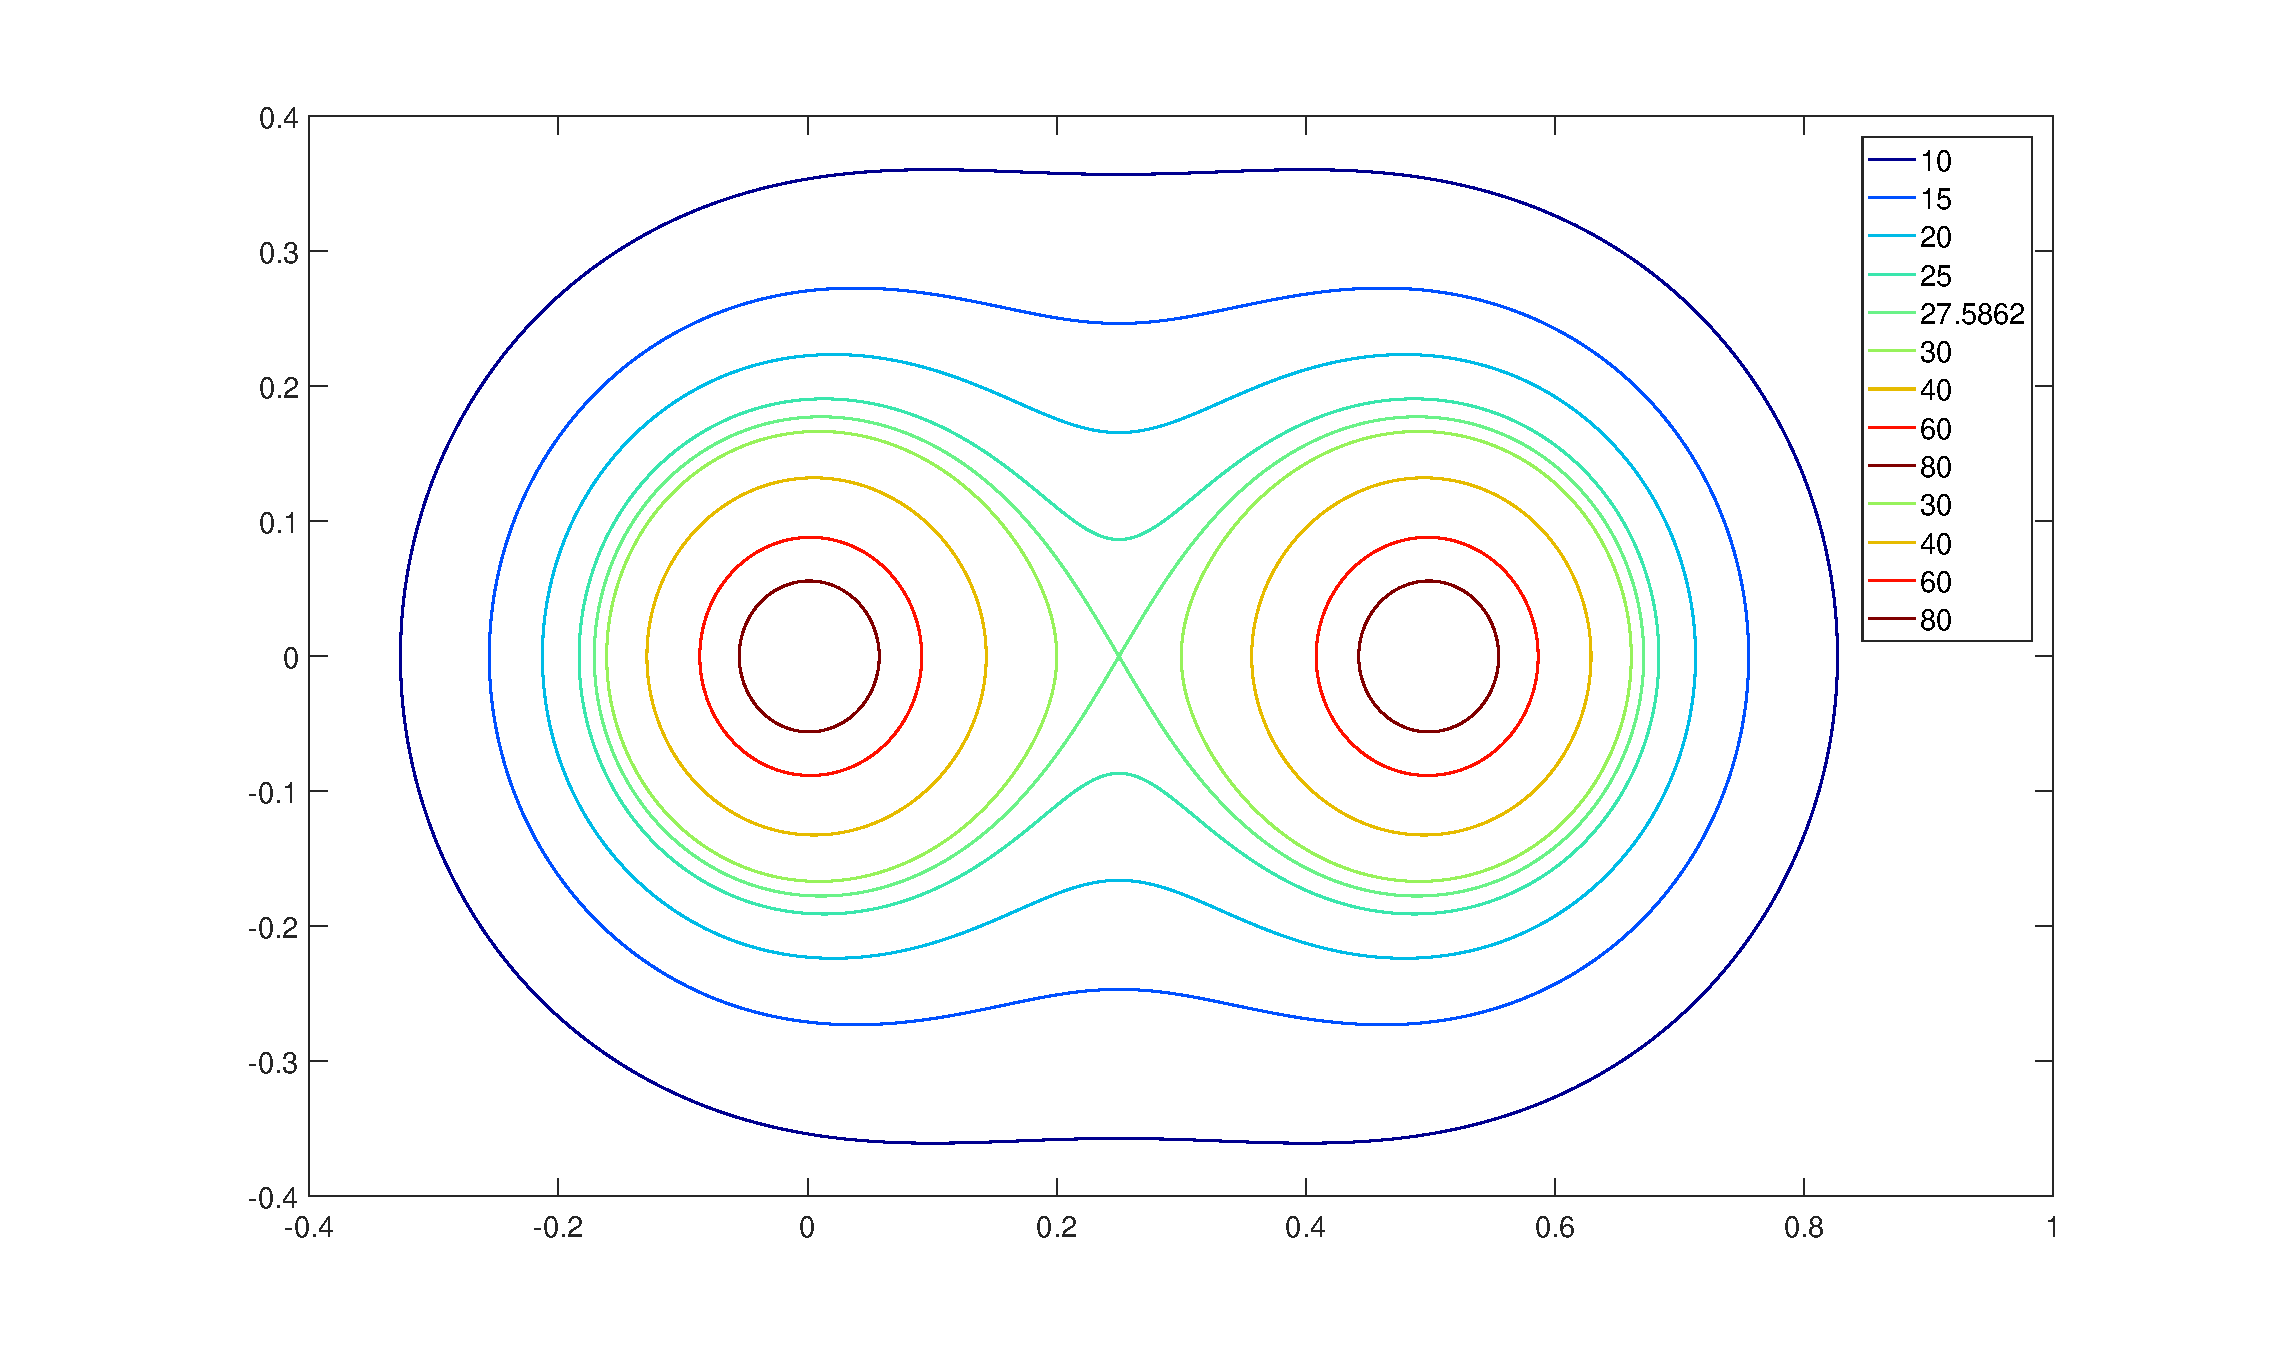
\includegraphics[trim = 41mm 0mm 35mm 0mm, clip, width=\linewidth]{plots/niveau/test5_}

\end{figure}

\section{Anhang: Code-Listings}
\lstinputlisting[firstline=1, lastline=1000,caption=Implementierung der Nullstellensuche im $\R^2$]{code/findZero.m}
%man wird wohl nur einzelne Ausschnitte im Fließtext haben wollen





\end{document}
